\chapter{Infraestructura}\label{chap:Infraestructura}
En este capítulo vamos a hablar de la infraestructura que da soporte a este proyecto, y las diversas herramientas que se han utilizado para realizarlo. Para esto, empezaremos explicando qué es JdeRobot, la plataforma en la que se enmarca VisualHFSM. A continuación, hablaremos de Gazebo y comentaremos la importancia de los simuladores en robótica. Después detallaremos qué es ICE, y finalizaremos comentando las distintas librerías gráficas utilizadas para elaborar la GUI, principalmente GTK+ y PyQt4, y la herramienta Glade.

%%%%%%%%%%%%%%% JdeRobot %%%%%%%%%%%%%%%
\section{JdeRobot}
Inicialmente la plataforma JdeRobot\footnote{\url{http://jderobot.org}}\cite{peredadocencia, canas2013recent} fue creada como resultado de una tesis doctoral, y ha sido mantenida y mejorada a largo de los años por el laboratorio de Robótica de la Universidad Rey Juan Carlos, un grupo voluntario de desarrolladores.  \\

JdeRobot es una plataforma de código libre pensada para facilitar la programación de aplicaciones de robótica y visión artificial. Es una plataforma orientada a componentes, con distintos elementos independientes. Estos componentes se ejecutan siguiendo un modelo cliente-servidor, en el que cada aplicación es ejecutada como un proceso, ofreciendo una interfaz para programar sistemas de tiempo real y resolver problemas que estén relacionados con la sincronización de procesos y la adquisición de datos. Tradicionalmente, los componentes estaban principalmente programados en C/C++, aunque en la actualidad la tendencia es utilizar el lenguaje Python. Sin embargo, hay programas en otros lenguajes, como por ejemplo, JavaScript. \\

JdeRobot simplifica el acceso a los sensores y actuadores (a los dispositivos hardware), permitiendo obtener valores y enviar datos de forma sencilla. Para esta interacción, utiliza como puente los interfaces de comunicación ICE. \\

Por último, comentar que todo el código y los componentes que se encuadran en esta plataforma puede encontrarse en GitHub\footnote{\url{https://github.com/RoboticsURJC/JdeRobot}}. La arquitectura se encuentra dividida en componentes, drivers, interfaces, librerías y herramientas. VisualHFSM se sitúa dentro de esta plataforma en la sección de herramientas, y es compatible con su última versión, JdeRobot 5.3.2.


%%%%%%%%%%%%%%% Gazebo %%%%%%%%%%%%%%%
\section{Gazebo}
A pesar de que la robótica es un campo que genera un gran interés, en ocasiones, la gran inversión necesaria para acceder al hardware puede resultar prohibitiva. Es por esto que la simulación por ordenador se plantea como una alternativa válida y de bajo coste. Sin embargo, la simulación ofrece otras ventajas adicionales que justifican su uso:

\begin{itemize}
\item \textsl{Gestión de recursos:} Utilizar un simulador combinado con una capa de abstracción al hardware (HAL), permite desarrollar código para robots existentes pero a los que no se tiene acceso en un determinado momento. Esto resulta especialmente útil cuando hay varios desarrolladores trabajando con un único robot.
\item \textsl{Control del tiempo:} Algunos simuladores (entre ellos, Gazebo), permiten modificar el tiempo, parándolo o acelerándolo, tanto negativa como positivamente. Esto resulta especialmente útil, por ejemplo, a la hora de hacer pruebas de durabilidad o para inspeccionar el estado de los robots en cierto momento.
\item \textsl{Prototipado:} Gracias a la simulación existe la posibilidad de crear software para robots que aún no han sido contruidos.
\item \textsl{Reusabilidad:} Como el uso de simuladores suele combinarse con algún tipo de capa de abstracción, el código generado puede ser compartido con otras personas.
\end{itemize}

Gazebo\footnote{\url{www.gazebosim.org}} es un simulador 3D que ofrece un entorno para desarrollar y probar sistemas multirrobot de manera sencilla\cite{koenig2004design}. Permite la simulación realista de gran variedad de sensores y actuadores como cámaras, láser, GPS, etc., gracias, en parte, al motor de física que utiliza, ODE (\textit{Open Dynamics Engine}), y a la librería gráfica OpenGL (\textit{Open Graphics Library}). Además, Gazebo da soporte a una gran variedad de robots comerciales como \emph{Turtlebot}, el \emph{Pioneer 2-DX} o el \emph{Ar Drone}, y es también una herramienta de software libre. \\

Este simulador nació dentro del proyecto Player/Stage, pero se acabó separando y está siendo mantenido por Open Source Robotics Foundation\footnote{\url{http://www.osrfoundation.org/}}, una empresa de I+D sin ánimo de lucro e independiente encargada de apoyar el desarrollo, la distribución y la adopción del código abierto en investigación con robots, educación y desarrollo de productos. Además, Gazebo ha recibido financiación de DARPA (\textit{Defense Advanced Research Projects Agency}), convirtiéndose así en el simulador estándar \textit{de facto} dentro de la comunidad robótica, siendo empleado también para el \textit{DARPA Robotics Challenge}. \\

Otra de las principales características de Gazebo es que permite crear nuevos modelos y mundos robóticos. Un mundo simulado en Gazebo es un conjunto de todos los modelos y factores ambientales, como al luz o la gravedad. Los modelos se componen de al menos un cuerpo, con las articulaciones que éste pueda necesitar. Cuando el modelo está listo, las aplicaciones robóticas se conectan al simulador mediante los \textit{plugins} o bibliotecas dinámicas. Es necesario implementar estas bibliotecas utilizando la API de Gazebo. En la figura \ref{fig:gazeboWorld} podemos observar uno de los mundos de Gazebo creados para un experimento.

\begin{figure}[htbp]
	\centering
	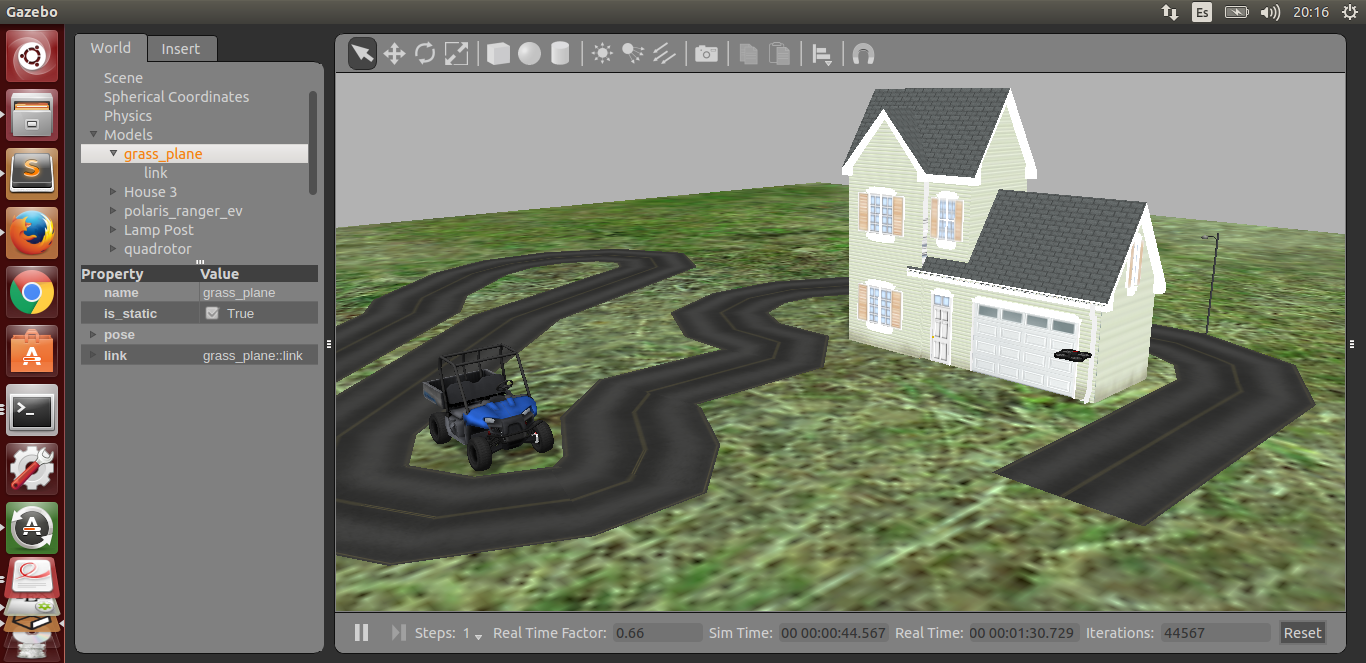
\includegraphics[height=7cm]{imgs/3_infrastructure/gazeboWorld.png}
	\caption{Mundo de Gazebo creado para realizar pruebas.}
	\label{fig:gazeboWorld}
\end{figure}

En este TFG hemos utilizado Gazebo 5.3 para simular los mundos de los experimentos y los robots que han ejecutado los componentes generados mediante VisualHFSM para comprobar su correcto funcionamiento.

%%%%%%%%%%%%%%% ICE %%%%%%%%%%%%%%%
\section{ICE}
ICE\footnote{\url{https://zeroc.com/}} es un \textit{middleware} desarrollado por ZeroC empleado por JdeRobot para la intercomunicación de componentes, especialmente importante para comunicarse con los \textit{drivers} que permiten la relación con los sensores y actuadores del robot. Es un entorno RPC (\textit{Remote Procedure Call}) orientado a objetos que provee de una capa de abstración sobre la red y sus conexiones, con una doble licencia GNU GPL y una licencia propietaria. \\

ICE permite utilizar aplicaciones de Internet sin la necesidad de usar los protocolos HTTP, y además, es capaz de atravesar cortafuegos, una característica que lo diferencia de la mayoría de los \textit{middleware} similares. Soporta  distintos sistemas operativos como Windows, MAC OS X, Linux y Solaris, y provee un IDE (\textit{Interface Definition Language}): SLICE (\textit{Specification Language for ICE}), que ayuda a definir la manera de comunicación y los parámetros utilizados entre los componentes. Una vez que dicho interfaz de comunicación está definido, se puede compilar en distintos lenguajes, dando así soporte a Python, C++, C\#, Java o JavaScript, entre otros. Además, esto hace que el cliente y el servidor puedan estar programados en distintos lenguajes. \\

Existe también una variante, ICE-E, que permite utilizar ICE dentro de teléfonos móviles. \\

Para nuestra herramienta hemos utilizado ICE 3.6 para que los componentes generados con VisualHFSM puedan comunicarse con los sensores y actuadores del robot.


%%%%%%%%%%%%%%% GTK+, Glade %%%%%%%%%%%%%%%
\section{GTK+}
Para la realización de este proyecto hemos utilizado diferentes librerías gráficas para diseñar la GUI en tiempo de ejecución. Para el componente generado en C/C++ hemos empleado la tercera versión de \emph{GTK+}. El principal motivo por el que hemos empleado esta librería, ha sido porque queríamos que el aspecto de la GUI en tiempo de ejecución fuese lo más parecido posible a la GUI del editor gráfico, y con la idea también de reutilizar y reestructurar todo el código posible del editor. \\

GTK+\footnote{\url{http://www.gtk.org}} o \textit{TheGIMP ToolKit} es un conjunto de bibliotecas multiplataforma que permiten desarrollar interfaces gráficas de usuario (GUI, \textit{Graphic User Interface}). GTK es una interfaz orientada a objetos para programadores de aplicaciones (API, \textit{Application Programming Interface}), escrita principalmente en C, aunque cuenta con enlaces a otros lenguajes de programación como C++, Python y C\#. \\

GTK+ se basa en las bibliotecas desarrolladas por el equipo de GTK+ y por el equipo de GNOME\footnote{\url{http://www.gnome.org}}:

\begin{itemize}
\item \textbf{GLib:} Se trata de una biblioteca de bajo nivel que envuelve la mayor parte de las funciones de la biblioteca estándar de C para manejar estructuras de datos, portabilidad, interfaces para funcionalidades de tiempo de ejecución como ciclos, hilos de carga dinámica o un sistema de objetos.
\item \textbf{GDK:} Es una biblioteca que actúa como intermediaria entre gráficos de bajo nivel y gráficos de alto nivel.
\item \textbf{ATK:} Una biblioteca que permite la creación de interfaces accesibles para gente discapacitada.
\item \textbf{Pango:} Permite el diseño y renderizado de texto, siendo esta biblioteca el núcleo para mejorar las fuentes y el texto en GTK+2.
\item \textbf{Cairo:} Biblioteca de renderizado avanzado de controles de aplicación.
\item \textbf{GTK:} La biblioteca principal que contiene los objetos y funciones necesarios para crear e interaccionar con la interfaz de usuario.
\end{itemize}

Con GTK+ cada elemento de la interfaz gráfica recibe el nombre de \textit{Widget}. Los \textit{widgtets} pueden representar botones, cuadros de diálogos, barras de deslizamiento, etc. Existe una gran multitud de \textit{widgets} distintos, pero todos ellos heredan de una misma clase, tal como se observa en la figura \ref{fig:treeViewHeritage}, en la cual podemos observar el esquema de herencia de la clase Gtk::TreeView.

\begin{figure}[htbp]
	\centering
	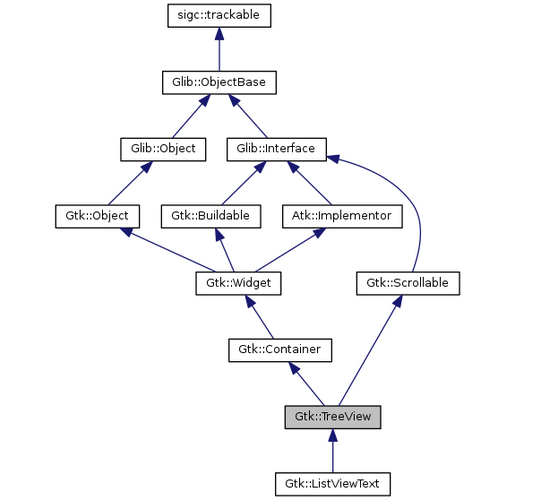
\includegraphics[height=6cm]{imgs/3_infrastructure/herenciaTreeView.png}
	\caption{Esquema de la herencia de la clase Gtk::TreeView.}
	\label{fig:treeViewHeritage}
\end{figure}

La forma de  interactuar con los \textit{widgets} es utilizando eventos. Cuando tiene lugar un evento, como hacer click en un \textit{widget} o cerrar una ventana, se emitirá una señal concreta. Esta señal puede ser conectada a una función (\textit{manejador} o \textit{callback}), de forma que cuando se emita dicha señal, se activará su manejador y se ejecutará el código que se haya programado dentro de él. De esta forma, para realizar una acción concreta cuando se pulse un botón, sólo es necesario programar dicha acción dentro de una función, y conectar la señal con ella. \\

\begin{figure}[htbp]
	\centering
	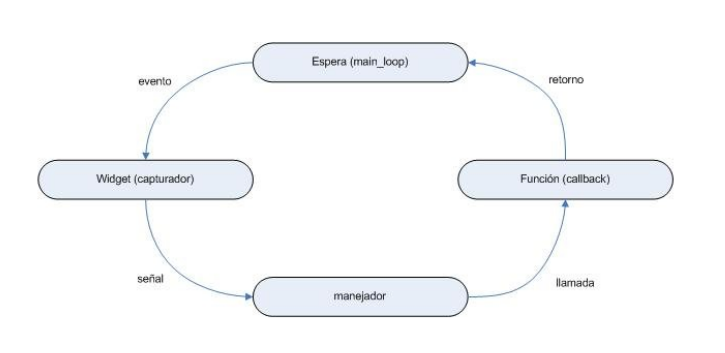
\includegraphics[height=6cm]{imgs/3_infrastructure/bucleGTK.png}
	\caption{Diagrama de flujo de GTK+.}
	\label{fig:gtkMain}
\end{figure}

Al trabajar con eventos, el diagrama de flujo de una aplicación GTK+ es como el que se observa en la figura \ref{fig:gtkMain}. Una vez arrancada, la interfaz gráfica se queda en un bucle a la espera de que se produzca un evento. Cuando esto sucede, el control lo recibe el \textit{callback} apropiado, y una vez que éste ha terminado, el control vuelve al bucle principal, que vuelve a quedar a la espera de que se produzca un evento nuevo. \\

Para el desarrollo de la interfaz gráfica con la librería GTK+ hemos utilizado \emph{Glade Interface Designer}\footnote{\url{https://glade.gnome.org/}}. Esta herramienta permite diseñar la interfaz gráficamente, guardándola en un fichero XML que puede cargarse dinámicamente en tiempo de ejecución gracias a los objetos \textit{GtkBuilder}. En la figura \ref{fig:gladeDesigner} podemos observar una captura de esta herramienta. \\

%Glade 
\begin{figure}[htbp]
	\centering
	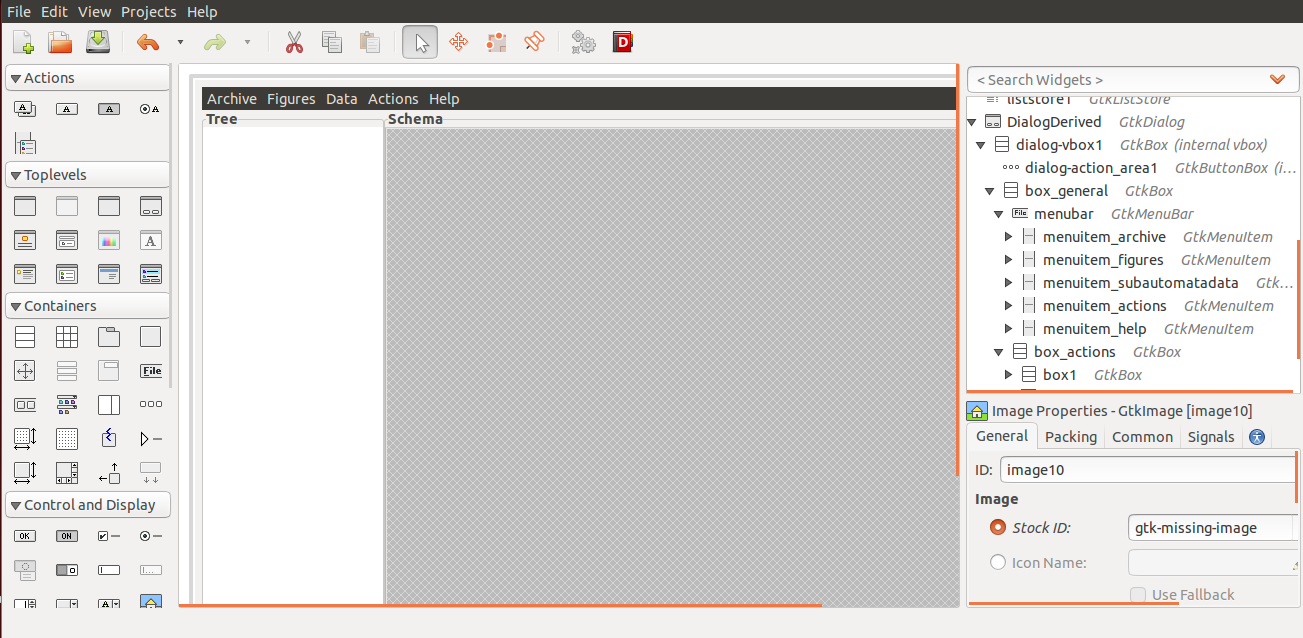
\includegraphics[height=6cm]{imgs/3_infrastructure/gladeEditor.png}
	\caption{Glade Interface Designer.}
	\label{fig:gladeDesigner}
\end{figure}


%%%%%%%%%%%%%%% PyQt4 y PyQt 4 Designer%%%%%%%%%%%%%%%
\section{PyQt4}
%PyQt4
Para el componente en Python, hemos optado por utilizar la versión 4 de PyQt, un \textit{binding} de la biblioteca gráfica Qt, desarrollada por Riverbank Computing\footnote{\url{https://riverbankcomputing.com/}} y disponible para Windows, GNU/Linux y Mac OS X bajo diferentes licencias. Este cambio de librería gráfica se debe principalmente a que al trabajar ahora con aplicaciones en Python, la reutilización del código del editor original, escrito en C++, ya no resulta importante. \\

Qt\footnote{\url{http://www.qt.io/}} es una biblioteca multiplataforma ampliamente utilizada para desarrollar aplicaciones con GUI, desarrollada como un software libre y de código abierto a través de Qt Project, donde participa tanto la comunidad, como desarrolladores de Nokia y Digia, entre otras empresas. Está hecho en C++, pero adicionalmente puede ser utilizado en otros lenguajes de programación mediante \textit{bindings}, estando disponible para Python, C\#, Ruby y Java, entre otros. \\

PyQt4 se encuentra dividido en una serie de componentes que pueden ser importados individualmente como módulos de Python, de los cuales hemos utilizado:

\begin{itemize}
\item \textbf{QtCore:} Contiene las clases que no están directamente relacionadas con la GUI, incluyendo el bucle principal de la interfaz y funciones para trabajar con señales y \textit{slots}.
\item \textbf{QtGui:} Módulo que contiene la mayoría de las clases relacionadas con la GUI.
\end{itemize}

En cuanto al flujo de ejecución, PyQt4 funciona igual que GTK+, quedándose a la espera de que se produzca un evento, y pasándole el control a su manejador cuando este tiene lugar, cómo ya hemos explicado. \\

% Qt 4 Designer
Para diseñar la GUI en tiempo de ejecución con PyQt4 hemos utilizado la herramienta \emph{Qt 4 Designer}, que puede observarse en las figura \ref{fig:qtDesigner}. Al igual que \textit{Glade}, permite realizar el desarrollo de la GUI de forma gráfica guardando el diseño en un archivo XML y permitiendo su carga dinámica en tiempo de ejecución. Sin embargo, nos hemos aprovechado de una de las herramientas que ofrece PyQt4: \textit{pyuic4}. Este programa convierte el archivo XML que se ha diseñado en código Python, de forma que puede importarse como un módulo más, evitando que esta traducción tenga lugar en tiempo de ejecución y minimizando así el tiempo de carga de la GUI. \\

\begin{figure}[htbp]
	\centering
	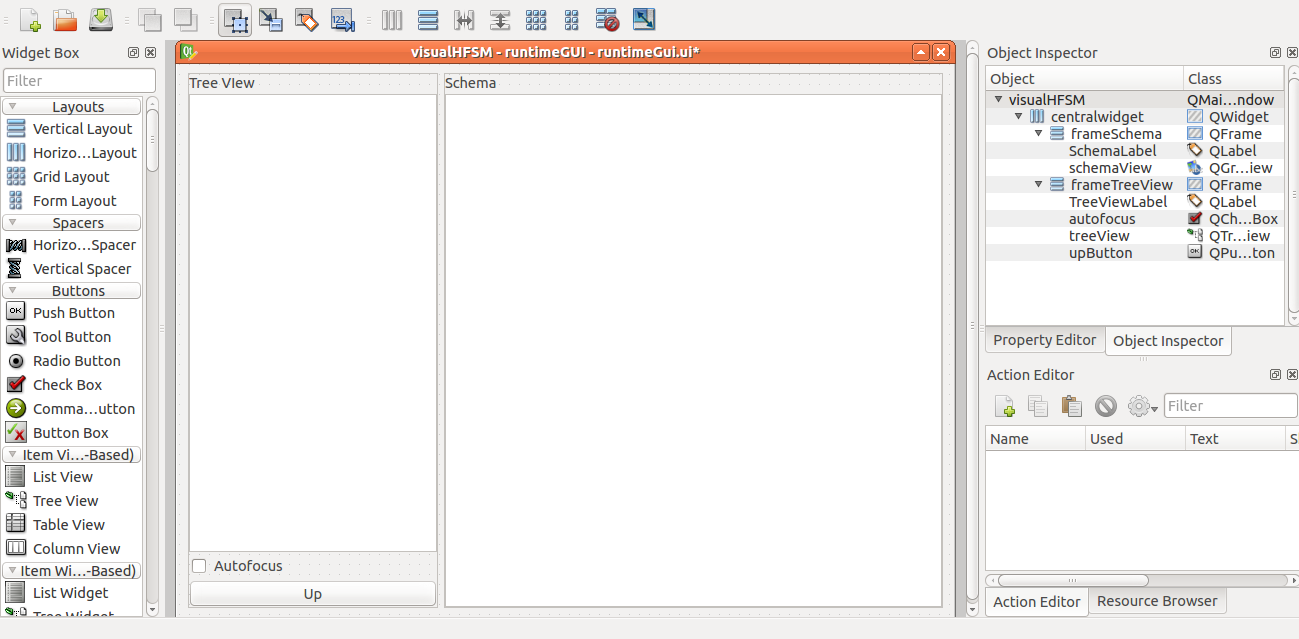
\includegraphics[height=6cm]{imgs/3_infrastructure/qtDesigner.png}
	\caption{Qt 4 Designer.}
	\label{fig:qtDesigner}
\end{figure}